\documentclass[12pt]{article}

\usepackage{listings}
\usepackage{graphicx,url}
\usepackage[utf8]{inputenc}
\usepackage[brazil]{babel}

\title{Trabalho Teórico 5}
\author{Iyan Lucas Duarte Marques}
\begin{document}
\maketitle
\section{Exercícios}
\subsection{Exercício 2 (p104)}
\begingroup
\LARGE
\begin{equation}
\sum_{1}^{m-3}a_i + \sum_{m}^{n}a_i = \sum_{1}^{n}a_i - a_{m-2} - a_{m-1}
\end{equation}
\endgroup
\subsection{Exercício 3}
Pior caso  $\Theta(n^2)$

Melhor caso: $\Theta(n)$

Caso médio para um arranjo aleatório: $\Theta(n^2)$

Caso de arranjo "quase ordenado": $\Theta(n)$
\section{Exercícios Resolvidos}
\subsection{Exercício 1}
Mostre o somatório dos n primeiros números inteiros
\begingroup
\LARGE
\begin{equation}
    \sum_{i=1}^{i\leq n}(a_i + b_i)
\end{equation}
\endgroup
\subsection{Exercício 2}
O Algoritmo de Seleção é uma solução conhecida para a ordenação
interna. Quantas comparações entre registros ele realiza?
\begingroup
\LARGE
\begin{equation}
    \sum_{i=0}^{n-2}(n-i-1)
\end{equation}
\endgroup
\subsection{Exercício 3}
\begingroup
\large

b)
\endgroup
\subsection{Exercício 4}
\begingroup
\large    
    (3 * 1) + (3 * 2) + (3 * 3) + (3 * 4) = 30
\endgroup
\subsection{Exercício 5}
\begingroup
\large
    
(3 - (2 . 1)) + (3 - (2 . 2)) + (3 - (2 . 3)) + (3 - (2 . 4)) = -8
\endgroup
\subsection{Exercício 6}
\begingroup
\large
2(1 + 2 + 3) + (x + x + x) = 12 + 3x
\endgroup
\subsection{Exercício 7}
\begingroup
\large
    
5 . 4 . 0 = 0 + 0 + 6 + 12 + 12 + 0 = 30
\endgroup
\subsection{Exercício 8}
Sim, pois como os termos a0, a1 e a5 são iguais a zero, o resultado dos dois somatórios é igual a (a2+ a3+ a4)
\subsection{Exercício 9}
\begingroup
\large  
b)
\endgroup
\subsection{Exercício 10}
\begingroup
\large  
a)
\endgroup
\subsection{Exercício 11}
\begingroup
\LARGE    
\begin{equation}
    b_1 + b_2 + \sum_{3}^{n}(a_i + b_i)
\end{equation}
\endgroup
\subsection{Exercício 12}
\subsubsection{a)}
\begingroup
\LARGE    
\begin{equation}
    \sum_{k=0}^{200}k^3 = \sum_{k=1}^{200}k^3
\end{equation}
\endgroup
Essa expressão é verdadeira pelo fato de $k_0^3 = 0$ e por isso não faz diferença
na soma.
\subsubsection{b)}
\begingroup
\LARGE    
\begin{equation}
    \sum_{p=0}^{1000}(3 + p) = 3 + \sum_{p=0}^{1000}p
\end{equation}
\endgroup
Essa expressão é falsa porque, no primeiro somatório, o 3 se repete 1000 vezes. Na segunda, o 3 não se repete.
\subsubsection{c)}
\begingroup
\LARGE    
\begin{equation}
    \sum_{l=1}^{n}(3l) = 3\sum_{l=1}^{n}l
\end{equation}
\endgroup
Essa expressão é verdadeira pela propriedade distributiva.
\subsubsection{d)}
\begingroup
\LARGE    
\begin{equation}
    \sum_{k=0}^{12}(k^p) = (\sum_{k=0}^{12}k)^p
\end{equation}
\endgroup
Essa expressão é falsa pelo fato de que a potência no primeiros somatório está elevando todo o k. Já no segundo, eleva somente o resultado do somatório.
\subsubsection{e)}
\begingroup
\LARGE    
\begin{equation}
    \sum_{t=8}^{32}(3 + t) = 75 + \sum_{t=8}^{32}t
\end{equation}
\endgroup
Essa expressão é verdadeira pelo fato de 75 ser 3 * 25.
\subsection{Exercício 13}
No primeiro somatório temos (3 + 2.0) + (3 + 2.1) + (3 + 2.2) + (3 + 2.3) +
(3 + 2.4) e no segundo, (3 + 2.[4-0]) + (3 + 2.[4-1]) + (3 + 2.[4-2]) + (3 +
2.[4-3]) + (3 + 2.[4-4]). Logo, por comutatividade, temos o mesmo
somatório alterando apenas a ordem dos elementos.
\subsection{Exercício 14}
Os valores a e b são 1 e 3, respectivamente, logo, temos:

1 + 3 . 0 = 1

1 + 3 . 1 = 4

1 + 3 . 2 = 7

1 + 3 . 3 = 10

1 + 3 . 4 = 13
\subsection{Exercício 15}
\begingroup
\LARGE    
\begin{equation}
    S_n = \sum_{0\leq i\leq n}[a + b * i] = \frac{(2a + bn)(n+1)}{2}
\end{equation}
\endgroup
\subsection{Exercício 16}
Nesse caso, temos uma progressão cujos valores a e b são
zero e um, respectivamente
\begingroup
\LARGE    
\begin{equation}
    S_n = \sum_{0\leq i\leq n}[0 + 1 * i] = \frac{(2*0 + n)(n+1)}{2} = \frac{n*(n+1)}{2}
\end{equation}
\endgroup
\subsection{Exercício 17}
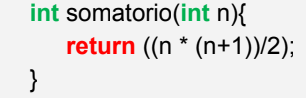
\includegraphics[width=7cm]{3.png}
\subsection{Exercício 18}
\begingroup
\LARGE    
\begin{equation}
    \frac{n^2}{2} - \frac{n}{2} = \Theta(n^2)
\end{equation}
\endgroup
\subsection{Exercício 19}
Os dois somatórios são iguais, entretanto, o segundo faz uma
soma a mais que é com seu primeiro termo cujo valor é zero.
\subsection{Exercício 20}
Os somatórios são diferentes, porque, não necessariamente,
o primeiro termo $(a_0)$ é igual a zero
\subsection{Exercício 21}
O resultado dos dois somatórios é $(a1+ a_2 + a_3 + ... + a_n)$
\subsection{Exercício 22}
O primeiro somatório desconsidera os termos $a_0, a_1, a_n$ cujo valor é zero.
\subsection{Exercício 23}
\begingroup
\LARGE    
\begin{equation}
S_n = \sum_{0\leq i\leq n}(i*2^i) = \frac{a-a*x^{n+1}}{1-x}
\end{equation}
\endgroup
\subsection{Exercício 24}
\begingroup
\LARGE    
\begin{equation}
S_n = \sum_{0\leq i\leq n}(i*2^i) = (n-1)*2^{n+1}+2
\end{equation}
\endgroup
\subsection{Exercício 25}
\begingroup
\LARGE    
\begin{equation}
\frac{n^2+7n+6}{2}
\end{equation}
\endgroup
\subsection{Exercício 26}
\begingroup
\LARGE    
\begin{equation}
2n^2+3n
\end{equation}
\endgroup
\subsection{Exercício 27}
\begingroup
\LARGE    
\begin{equation}
10n^2+10n
\end{equation}
\endgroup
\subsection{Exercício 28}
\begin{enumerate}
    \item Passo base:
        \begingroup
        \LARGE    
        \begin{equation}
            (0-1)2^{0+1}+2=0
        \end{equation}
        \endgroup
        \item indução propriamente dita:
        \begingroup
        \LARGE    
        \begin{equation}
            S_n = (n-1)2^{n+1}+2
        \end{equation}
        \endgroup
\end{enumerate}
    \subsection{Exercício 29}
    \begingroup
    \LARGE    
    \begin{equation}
        S_n = \frac{n(n+1)(2n+1)}{6}
    \end{equation}
    \endgroup
\end{document}